%!TEX root = ../thesis.tex

\chapter{Method}

\section{Implementation}
A common application where GPGPU is used is when computing calculation heavy simulations such the N-Body problem described in this thesis, other common visualizations where GPGPU can be applied is to visualize fractals such as the Julia or Mandelbrot set, named after the french mathematician Gaston Julia and Benoit Mandelbrot. GPGPU has also been used in medicine for accelerated medical image reconstruction \cite{archirapatkave2011gpgpu}, as well as accelerating the Marching Cubes algorithm \cite{johansson2006accelerating}. 

This section describes the implementation of the visualization and the parallel N-Body algorithm in all discussed frameworks, as well as how the measurements were performed and what framework specific features was used. All implementations was implemented in C/C++. The visualization was implemented in the cross-platform API OpenGL on a Windows PC.

\section{Visualization}

Although not necessary for the evaluation, a visualization of the system was implemented. This was the first step in the implementation process, and the visualization was made using OpenGL. The purpose of the visualization is to make it easier to test and debug the application, which is very difficult without a proper way of visualizing the calculated positions. The N-Body visualization is very similar to a particle system, where each body is represented by a particle. To be able to visualize a very large amount of bodies, the visualization performance is critical, and there are a few ways of implementing a particle system in OpenGL.

The first, and perhaps the most intuitive way is to render a sphere in all positions, by calling \lstinline{glDrawArrays} N times e.g. in a for-loop. This is very inefficient in two regards; a sphere requires a lot of vertices to appear smooth, and drawing a large amount of spheres requeries a very large amount of vertex data. The second reason this is inefficient is because all SM's on the GPU will be dedicated to drawing a single polygon, resulting in a huge amount of performance loss. The solution to the first problem is fairly easy. Since the particles are so small, they don't have to be rendered with a high resolution. A commonly used trick when rendering particle systems is to represent each particle as a quad with a semi-transparent texture with a circle. Each particle will thus only consist of four vertices, which is far less than if each particle was represented by a sphere. The quad is then rotated so that the quad's normal always faces the camera, giving the illusion that the particle is actually a sphere (or whatever shape the texture represents). This technique is known as \textit{billboarding}.

The solution to the second problem is a bit more complex, and a few solutions exists.
One way is to generate a single vertex buffer object (VBO) with all the particles in them. This is a easy and effective solution that works on all platforms. 

The second way is to use geometry shaders to render a particle in each position. This is a great solution, the downside to this is that geometry shaders is only supported in systems with OpenGL version 3.2+, and is thus not very portable. 

The third way is to use instancing, meaning that a single mesh is used, but many instances of the mesh. This solution has a nice balance between performance and availability and was thus chosen in this implementation. To achieve this, two main VBO's are used: one VBO containing the positions of the quad, i.e. four vertex coordinates, and a second VBO of size $n$ containing the positions of the instances of the quad, where $n$ is the number of instances. The quad is then rendered using \lstinline{glDrawArraysInstanced(GL_TRIANGLE_STRIP, 0, 4, n)} \cite{OpenCLDocs}, where the first parameter states that the object should be rendered as a triangle strip, i.e. a series of connected triangles, sharing vertices. The second parameter specifies the starting index in the enabled arrays. The third parameter specifies the number of indices to be rendered, and the fourth the number of instances. The quad positions are passed to the vertex shader as a attribute, and the shader then translates the quad into its position. The result of the implementation can be seen in figure \ref{fig:OpenGLEarlyVis}, where $n=3.5 \times 10^6$, running at a stable ~60fps on a Nvidia GTX970 GPU. Each quad is rendered in a random $(x,y,z)$ position in a given bounding box.


\begin{figure}[!htpb]
    \centering
    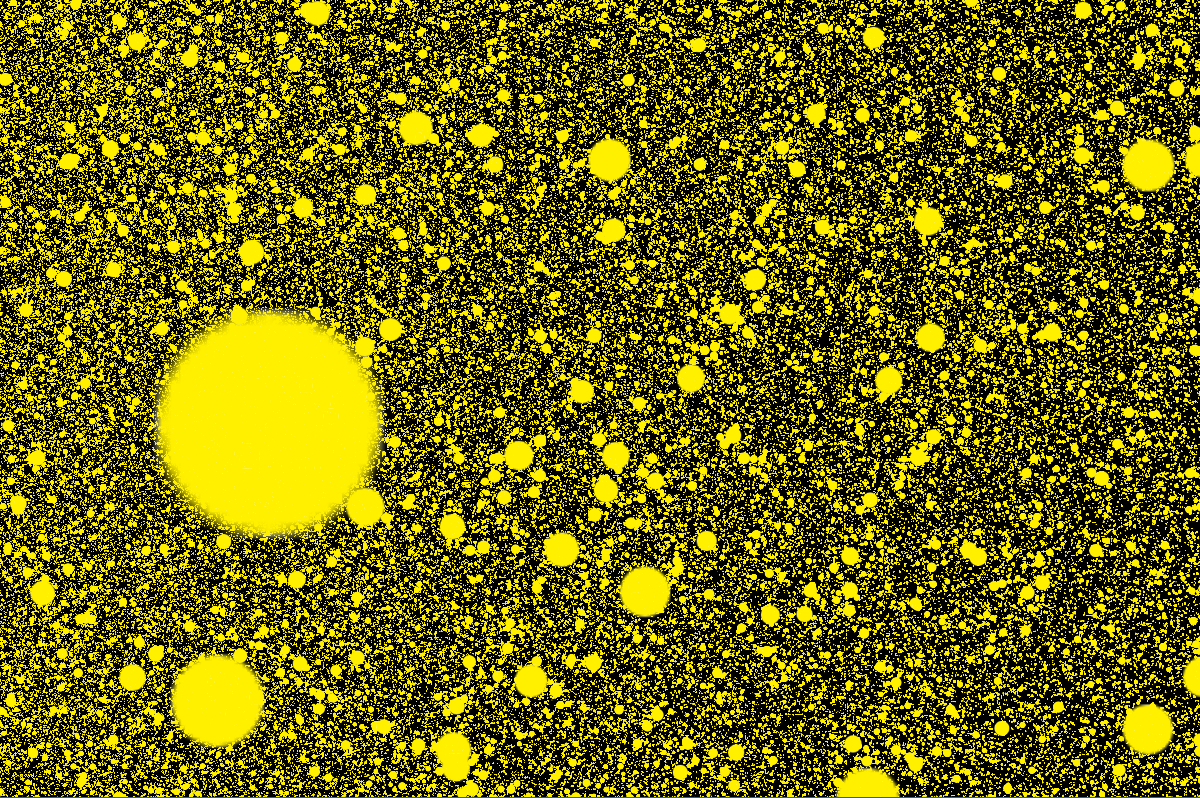
\includegraphics[width=0.8\textwidth]{Method/Figs/OpenGLVis_N=3500000.png}
    \caption{Instanced quad rendering, N=3.5*10^6}
    \label{fig:OpenGLEarlyVis}
\end{figure}


\section{CUDA}

\subsection{Tree-construction}

\section{OpenCL}

\section{SkePU}

\nomenclature[z-VBO]{VBO}{Vertex Buffer Object}